\section{Realizacja testów i analiza ich wyników}

Po zmodyfikowaniu podzespołu należy sprawdzić, czy oryginalna funkcjonalność nie została w jakiś sposób naruszona oraz dodana funkcjonalność działa zgodnie z założeniami. W tym celu podzespół należy poddać procesowi weryfikacji. Można jej dokonać na różne sposoby, zaczynając od testów jednostkowych i integracyjnych, kończąc zaś na weryfikacji formalnej.
Weryfikacja formalna jest dokładniejsza ze względu na wykorzystywanie formalnych metod matematycznych. Jednocześnie narzędzia, które wykorzystują tę metodę weryfikacji, są mało popularne i mogą nie być udokumentowane w wystarczającym stopniu. Wobec tego zostanie wykorzystana prostsza metoda testów jednostkowych --- polega ona na opisaniu sekwencji sygnałów wejściowych testowanego komponentu oraz instrukcji pozwalających na interpretację stanów wyjściowych poprzez porównywanie ich do oczekiwanych wzorców.
Testy jednostkowe są często używane przy tworzeniu nowoczesnego oprogramowania komputerowego, przez co narzędzia wykorzystywane w tym procesie są dobrze udokumentowane.

\subsection{Analiza i porównanie przebiegów aktywności magistrali}

Wspomniane testy jednostkowe zostaną wykorzystane w kontekście tej pracy do sprawdzenia, czy dane są poprawnie odczytywane i zapisywane w pamięci Block RAM z wykorzystaniem zarówno klasycznych, jak i potokowych cykli operacji na magistrali Wishbone. W tym celu każdy test wygeneruje sekwencję słów oraz adresów docelowych, które będą wykorzystywane do wytworzenia sygnałów wejściowych, jak i jako wzorzec, do którego będzie porównywany stan końcowy testowanej pamięci.
Ze względu na to, iż obserwujemy wyłącznie stan zewnętrzny, do pamięci Block RAM dostanie dodany drugi port, który będzie pozwalał na dokonywanie operacji na pamięci z pominięciem interfejsu Wishbone.

\subsubsection{Implementacja testów jednostkowych dla peryferiów}

Testy zostały zrealizowane z użyciem języka Python, wykorzystując bibliotekę Cocotb, która umożliwia tworzenie środowiska testowego z użyciem składni języka Python zamiast w języku Verilog. Pozwala to na integrację z bibliotekami ekosystemu języka Python, ułatwiając takie sprawy jak generowanie testowego zbioru danych.
Oprócz tego wykorzystane zostały biblioteki cocotb-test\cite{cocotb-test} oraz cocotbext-wishbone. Cocotb-test integruje Cocotb z systemem testów automatycznych pytest\cite{pytest6.2}, dzięki czemu napisane testy można uruchamiać z różnymi ustawieniami, co w połączeniu z parametryzacją samych testów umożliwia pokrycie różnych sposobów komunikacji z testowanym podzespołem na magistrali. Cocotbext-wishbone zaś implementuje funkcje do sterowania i monitorowania sygnałów na magistrali Wishbone, co pozwala zaoszczędzić czas poprzez wywoływanie gotowych funkcji realizujących operacje na magistrali zamiast poprzez ręczne sterowanie szyną.

\begin{figure}[H]
    \centering
    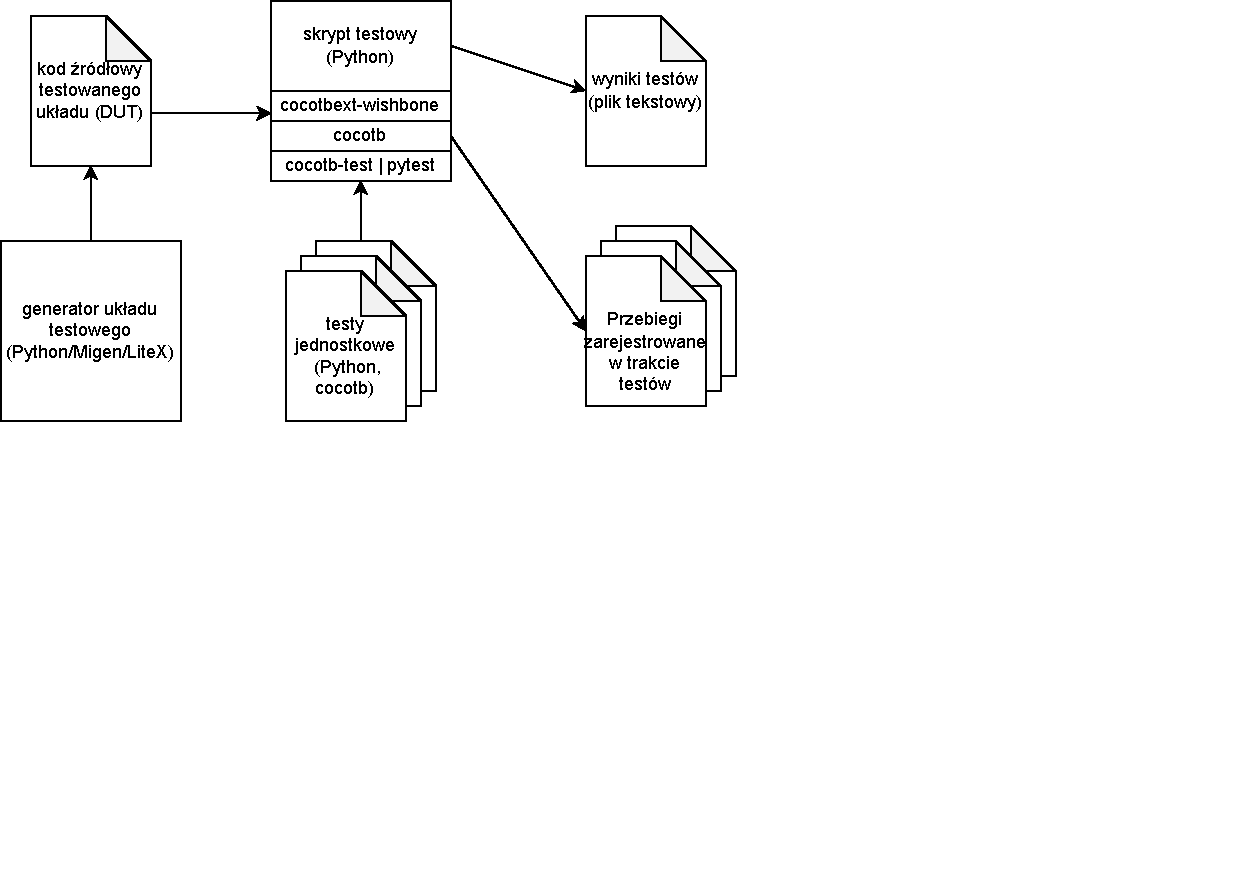
\includegraphics[scale=1,trim={0 7.7cm 8.5cm 0},clip]{testing/testing-pipeline.pdf}
    \caption{Schemat systemu testów jednostkowych zbudowany z wykorzystaniem biblioteki \texttt{cocotb}}
    \label{fig:testing-pipeline}
\end{figure}

Testowane peryferia, czyli pamięć SRAM oraz moduł transmisyjny, zostały zainstancjonowane w minimalnym module LiteX, który na zewnątrz udostępnia wspólną magistralę Wishbone, drugi port pamięci SRAM, wyjście nadawczej kolejki FIFO (First In, First Out) oraz wejście odbiorczej kolejki FIFO. W ten sposób mamy dostęp do wszystkich sygnałów, które posłużą do wysterowania magistrali oraz komunikacji z peryferiami inną drogą, umożliwiając obserwowanie wpływu implementacji interfejsu Wishbone na komunikację z peryferiami. Dzięki bezpośredniemu dostępowi do badanych peryferiów, z wykorzystaniem dodatkowych sygnałów (przykładowo drugi port pamięci RAM), możliwym było również wstępne zapisanie danych testowych do peryferiów oraz odczytanie wynikowych danych w celu sprawdzenia poprawności transferu danych. Jako że biblioteka Cocotb oczekuje opisu układu w języku Verilog, moduł LiteX jest przetwarzany do formy kodu w języku Verilog przed rozpoczęciem wykonywania testów.

\begin{longlisting}
\begin{minted}{python}
# wycięte: klasa _CRG definiująca wyprowadzenia modułu głównego
class BaseSoC(SoCCore):
    # wycięte: opis przerwań i adresów startowych peryferiów

    def __init__(self, platform, output_dir="build", **kwargs):
        self.output_dir = output_dir

        clk_freq = int(12e6)
        self.submodules.crg = _CRG(platform)

        # Inicjalizacja podstawowego szkieletu systemu jednoukładowego
        SoCCore.__init__(self, platform, clk_freq,
                         cpu_type=None, integrated_rom_size=0x0,
                         integrated_sram_size=0x100,
                         bus_bursting=True,
                         integrated_main_ram_size=0x0,
                         csr_address_width=14, csr_data_width=32,
                         with_uart=False, with_timer=False
                         )

        # Klasa definiująca minimalny mostek magistrali Wishbone
        class _WishboneBridge(Module):
            def __init__(self, interface):
                self.wishbone = interface

        sim_wishbone = wishbone.Interface()

        # Połączenie systemowej magistrali poprzez mostek
        # do sygnałów modułu głównego
        wb = self.platform.request('wishbone')
        copy_layout_directions(source=sim_wishbone, target=wb)
        self.comb += wb.connect(sim_wishbone)
        self.add_wb_master(sim_wishbone)

        # Dodanie drugiego portu do testowanej pamięci SRAM
        # i wyprowadzenie jego sygnałów
        sram_pins = self.platform.request('sram')
        sram_port = self.sram.mem.get_port(write_capable=True)
        self.specials += sram_port
        self.comb += [
            sram_port.adr.eq(sram_pins.adr),
            sram_port.dat_w.eq(sram_pins.dat_w),
            sram_pins.dat_r.eq(sram_port.dat_r),
            sram_port.we.eq(sram_pins.we),
        ]

        # Dodanie dwukierunkowego modułu FIFO
        # i wyprowadzenie sygnałów wejściowych i wyjściowych
        fifo_pins = self.platform.request('fifo')
        self.submodules.fifo = TestFIFOTransceiver(fifo_pins, 8)
        self.add_memory_region("fifo", self.mem_map["fifo"],
            self.bus.data_width//8, type=[]
            )
        self.add_wb_slave(self.mem_map["fifo"], self.fifo.bus)
\end{minted}
\caption{\label{lst:harness-basesoc}Fragment skryptu w języku Python generującego minimalny układ z testowanymi peryferiami oraz magistralą Wishbone}
\end{longlisting}

\subsubsection{Procedura wykonywania testów}
Zbiór testów jest wykonywany z użyciem komendy \texttt{pytest}, która jest częścią biblioteki o tej samej nazwie. Według definicji testów z pliku test.py generowana jest lista testów z różnymi kombinacjami parametrów według podanych przedziałów, przykładowo rozmiaru testowanego obszaru pamięci oraz przesunięcia pierwszego używanego adresu. Dzięki temu z czterech rodzajów testów (cykl klasyczny oraz wybrany cykl potokowych dla każdego peryferium) otrzymano zbiór 116 testów, które zostają wykonywane po kolei. Po zakończeniu testów program \texttt{pytest} zwraca ich wyniki, które można zapisać również w formacie HTML. Umożliwia to wychwycenie przypadków, dla których testy nie kończą się zgodnie z oczekiwaniami.

Poniżej zamieszczony jest przykładowy test, który wykonywuje operację odczytu dowolnej ilości słów, zaczynając od wybranego adresu. Dzięki sparametryzowaniu każdego testu możliwym jest uruchomienie tego samego testu z różnymi parametrami wejściowymi. Wykorzystując wypełnienie pamięci SRAM lub wejściowej kolejki FIFO losowymi danymi, możliwym było weryfikowanie poprawności transmisji poprzez porównywanie wynikowych danych ze wzorcem.

\begin{longlisting}
\begin{minted}{python}
@cocotb.test()
async def test_read(dut):
    # Parametry wejściowe, które mogą zostać zmodyfikowane przez skrypt:
    # adres startowy peryferium
    adr_base = int(os.environ.get("adr_base", "3489660928"))
    # przesunięcie adresu, od którego zacząć test
    adr_offset = int(os.environ.get("adr_offset", "0"))
    # inkrementacja adresu
    adr_inc = int(os.environ.get("adr_inc", "0"))
    # ilość słów do odczytania
    length = int(os.environ.get("length", "4"))
    # ilość losowych słów do zapełnienia pamięci SRAM
    sram_fill = int(os.environ.get("sram_fill", "0"))
    # ilość losowych słów do zapełnienia wyjściowej kolejki FIFO
    fifo_fill = int(os.environ.get("fifo_fill", "0"))

    # Przygotowanie danych testowych
    test_data = random.sample(range(0x80000000, 0xffffffff), length)
    ops_read = []
    for i in range(length):
        ops_read.append((adr_base+adr_offset+(i*adr_inc), None))

    # Przygotowanie środowiska
    harness = WbMaster(dut)
    clk_gen = make_clock(harness.dut, 100)

    # Kroki testu
    await harness.reset()
    if fifo_fill:
        await harness.fifo_write(test_data)
    if sram_fill:
        await harness.sram_write(adr_offset, test_data)
    responses = await harness.wb_classic_cycle(ops_read, acktimeout=3)

    clk_gen.kill()

    harness.count_cycles(responses)

    # Weryfikacja wyników
    for i in range(len(responses)):
        harness.dut._log.info("{} @ {:08x} ? {}".format(hex(responses[i].datrd), responses[i].adr, bin(test_data[i])))
        assert responses[i].datrd == test_data[i]
\end{minted}
\caption{\label{lst:harness-sampletest}Fragment testu w języku Python realizującego operację odczytu wybranej ilości słów poprzez magistralę Wishbone}
\end{longlisting}

\subsubsection{Porównanie wyników testów}

Na podstawie przebiegów wygenerowanych w trakcie wykonywania testów zauważyć można kilka różnic, które wpływają na wydajność transferów danych. Pierwszym z nich jest mniejsza ilość cykli zegarowych, w których trakcie przesłana została określona ilość słów po magistrali.
Na rysunkach \ref{fig:test-fifo-classic-8} oraz \ref{fig:test-fifo-constant-8} przedstawione zostały przebiegi dla dwóch testów: zapisu ośmiu losowych, 32-bitowych słów z użyciem klasycznego cyklu oraz cyklu potokowego ze stałym adresem. Główną różnicą między tymi przebiegami jest fakt, że w cyklu potokowym każde kolejne słowo było przekazywane w ciągu jednego cyklu zegara. Jest to spowodowane tym, iż ze względu na brak dodatkowych opóźnień moduł transmisyjny był w stanie obsłużyć transfer w każdym cyklu zegara, o czym informował utrzymywany w stanie wysokim sygnał \texttt{ACK}. Strona inicjująca połączenie również nie wymagała dodatkowych opóźnień przy transferze, co było sygnalizowane sygnałem \texttt{STB} będącym w stanie wysokim przez cały czas transmisji.

\begin{figure}[H]
	\centering
	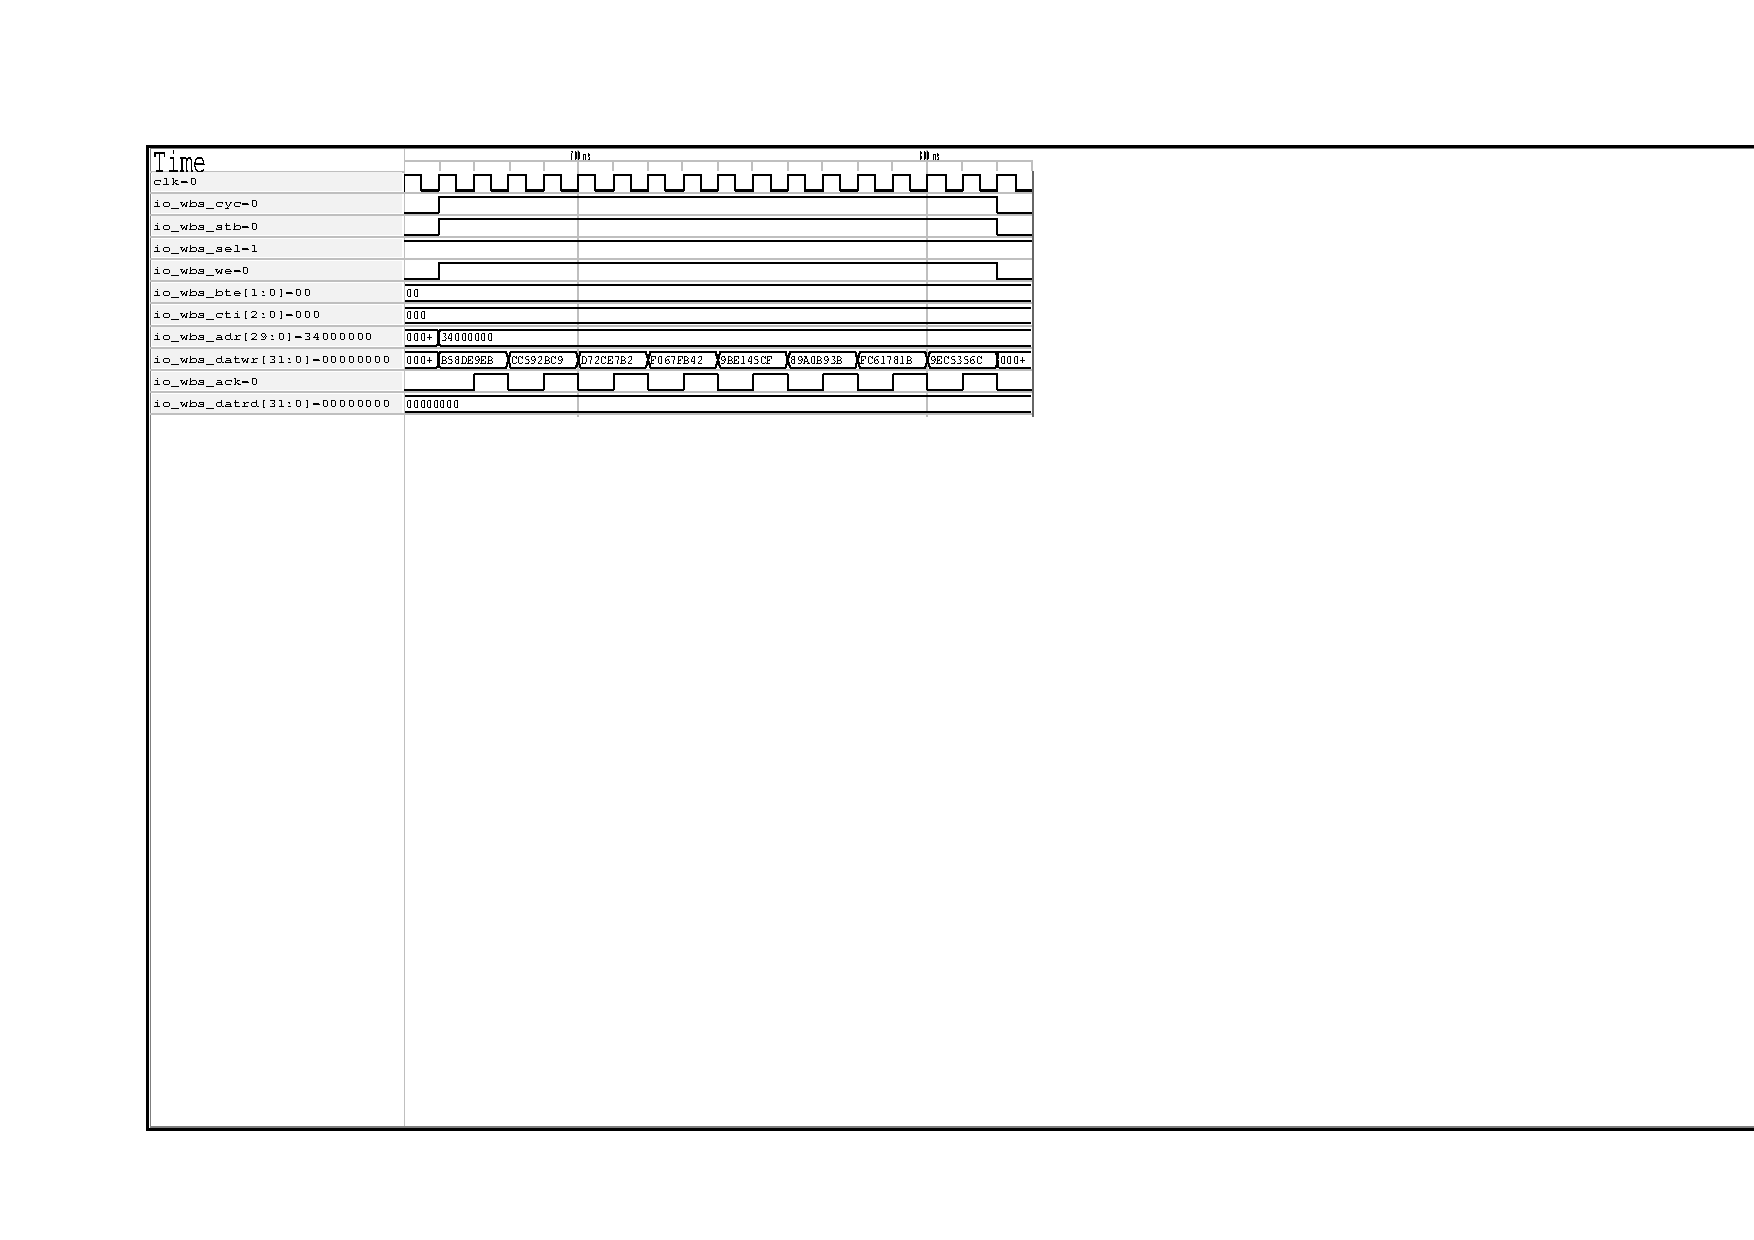
\includegraphics[scale=1,trim={2.54cm 14cm 12.3cm 2.9cm},clip]{testing/test-fifo-classic-8.pdf}
	\caption{Przebieg transferu danych do peryferium transmisyjnego w klasycznym cyklu magistrali Wishbone}
	\label{fig:test-fifo-classic-8}
\end{figure}

\begin{figure}[H]
	\centering
	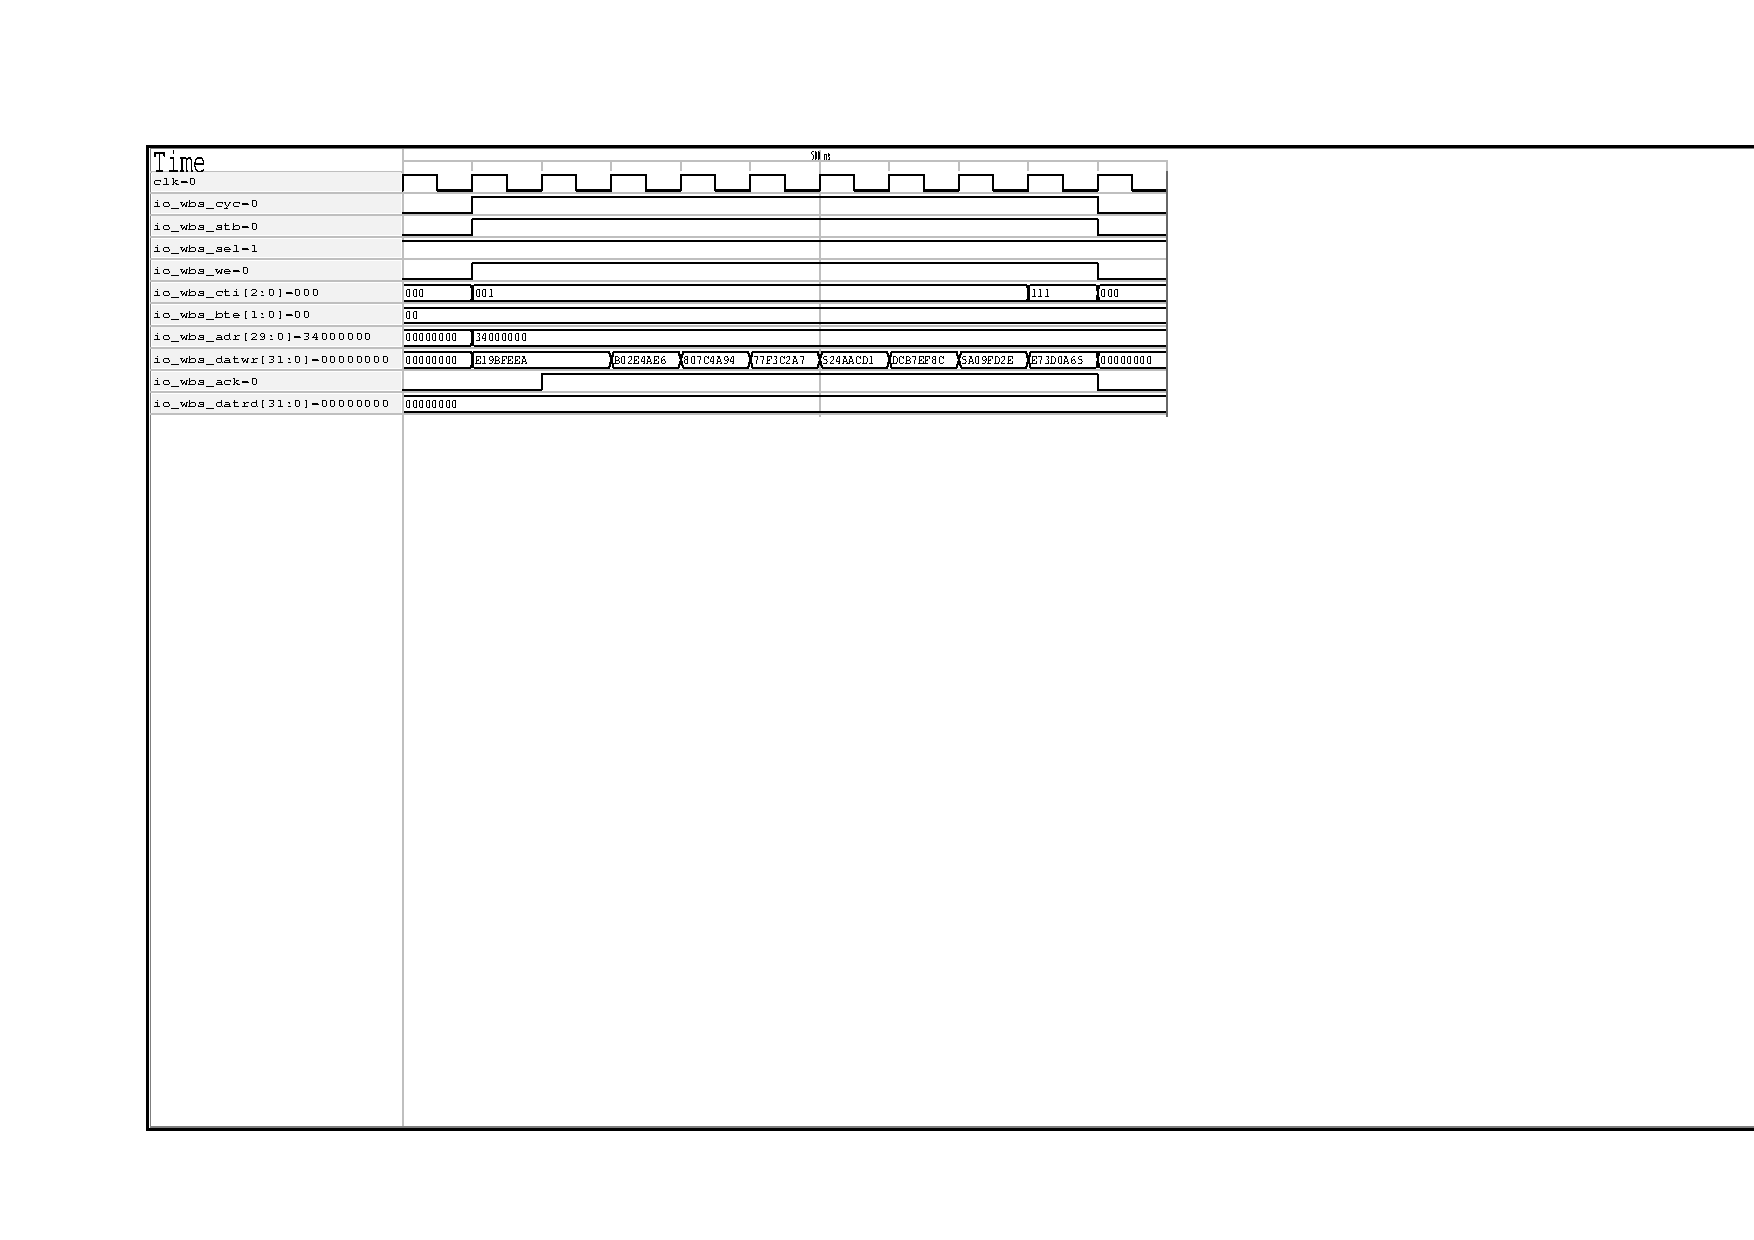
\includegraphics[scale=1,trim={2.54cm 14cm 11.1cm 2.9cm},clip]{testing/test-fifo-constant-8.pdf}
	\caption{Przebieg transferu danych do peryferium transmisyjnego w cyklu potokowym ze stałym adresem magistrali Wishbone}
	\label{fig:test-fifo-constant-8}
\end{figure}

W celu sprawdzenia poprawności transmisji dane zostaną odebrane z kolejki transmisyjnej poprzez zewnętrzne sygnały modułu FIFO. W tym celu zostały porównane odebrane słowa, przedstawione na przebiegu z rysunku \ref{fig:test-fifo-valid-8}, ze słowami zapisywanymi na przebiegu z rysunku \ref{fig:test-fifo-constant-8}. Ich wartości oraz kolejność są identyczne, co pozwala stwierdzić, że dane zostały przetransferowane w nienaruszonym stanie poprzez interfejs magistrali modułu oraz że jego część nadawcza, czyli kolejka FIFO działa poprawnie.

\begin{figure}[H]
	\centering
	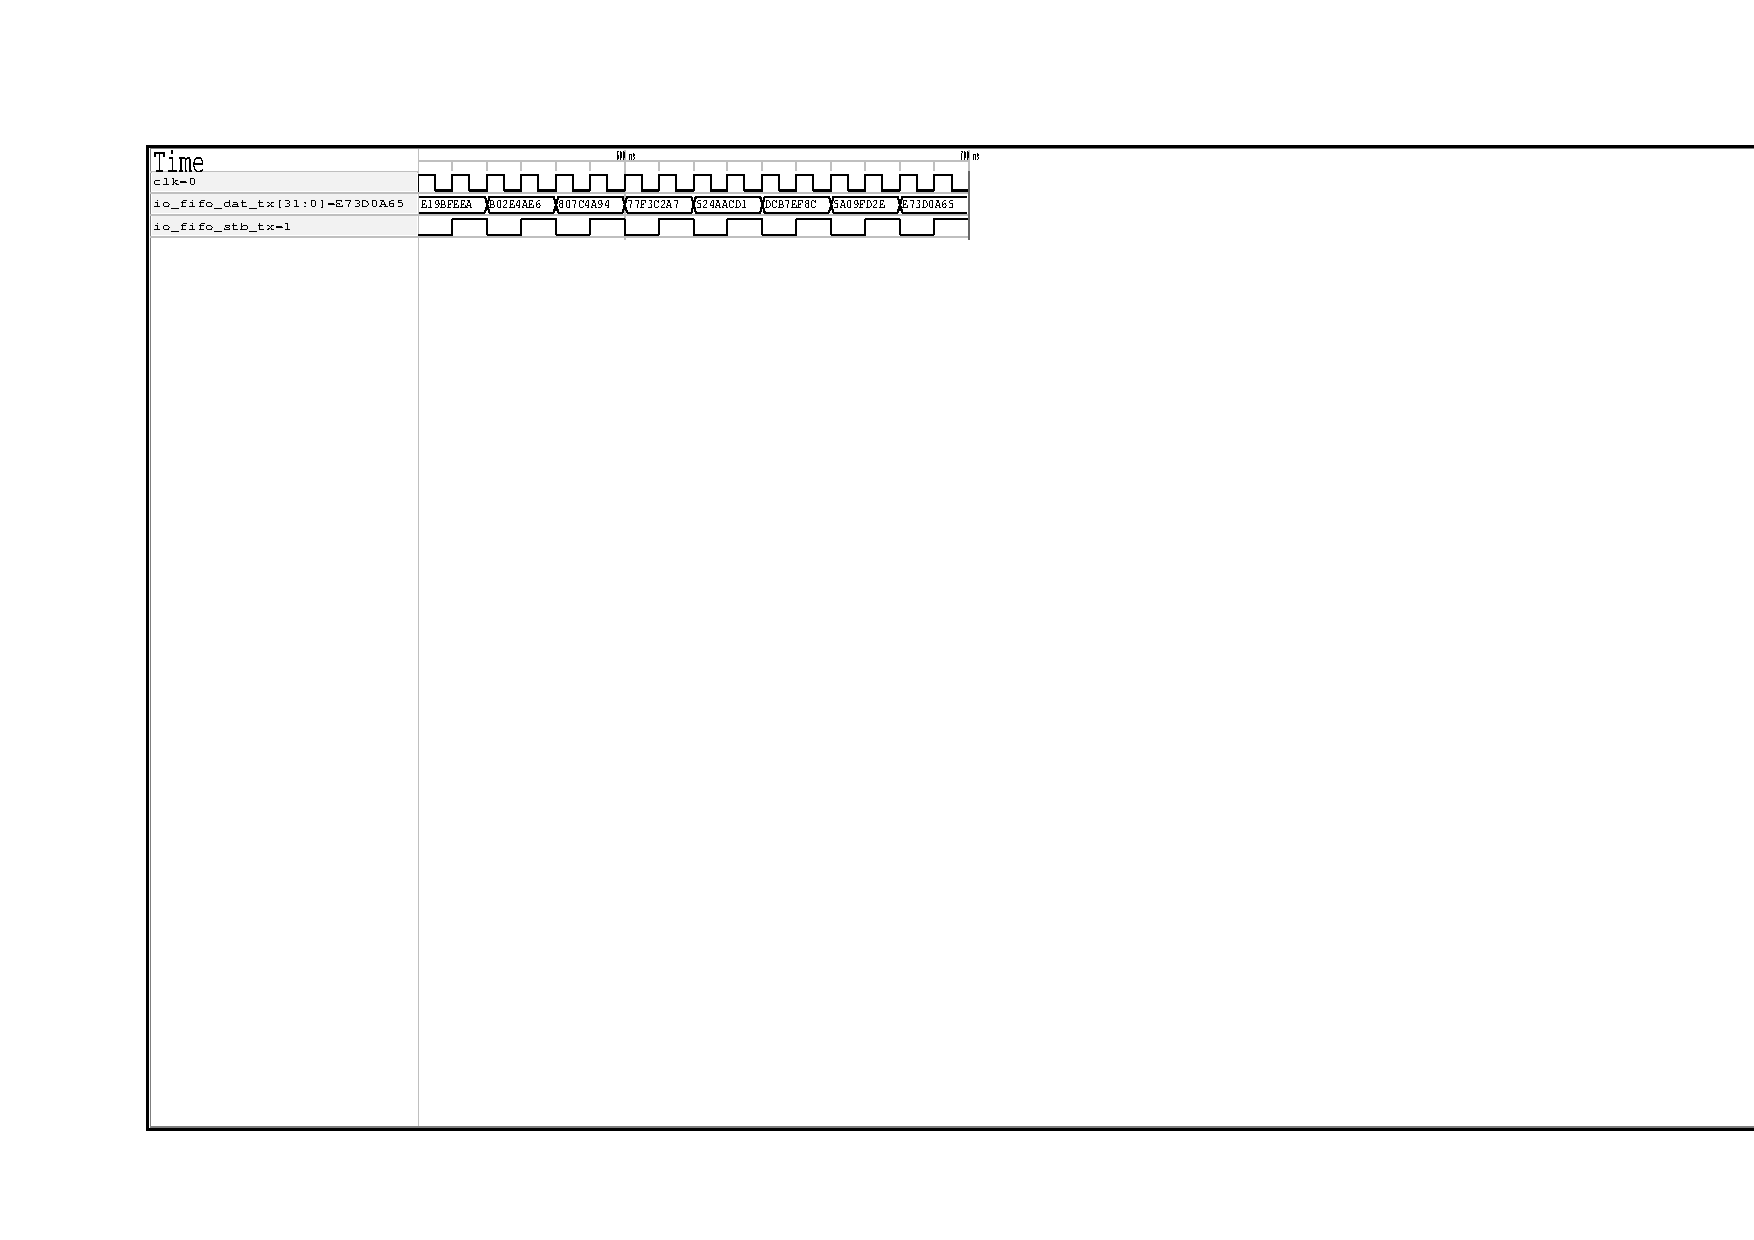
\includegraphics[scale=1,trim={2.54cm 17cm 13.3cm 2.9cm},clip]{testing/test-fifo-valid-8.pdf}
	\caption{Przebieg przedstawiający odczyt danych z kolejki nadawczej FIFO z użyciem sygnałów zewnętrznych}
	\label{fig:test-fifo-valid-8}
\end{figure}

Tę samą różnicę w prędkości transmisji zauważyć można również na przebiegach przedstawiających transfer danych z użyciem cykli potokowych z inkrementacją adresu. Na przebiegach z rysunków \ref{fig:test-sram-classic-8} oraz \ref{fig:test-sram-increment-8}, przedstawione zostały cykle odczytu ośmiu słów do pamięci SRAM, która poprzednio została zapełniona wygenerowanymi losowo danymi.
Widoczna jest identyczna różnica jak w poprzednio porównanych przebiegach, czyli transfer drugiego słowa i kolejnych zachodzący w czasie krótszym przy zastosowaniu transferu potokowego.

\begin{figure}[H]
	\centering
	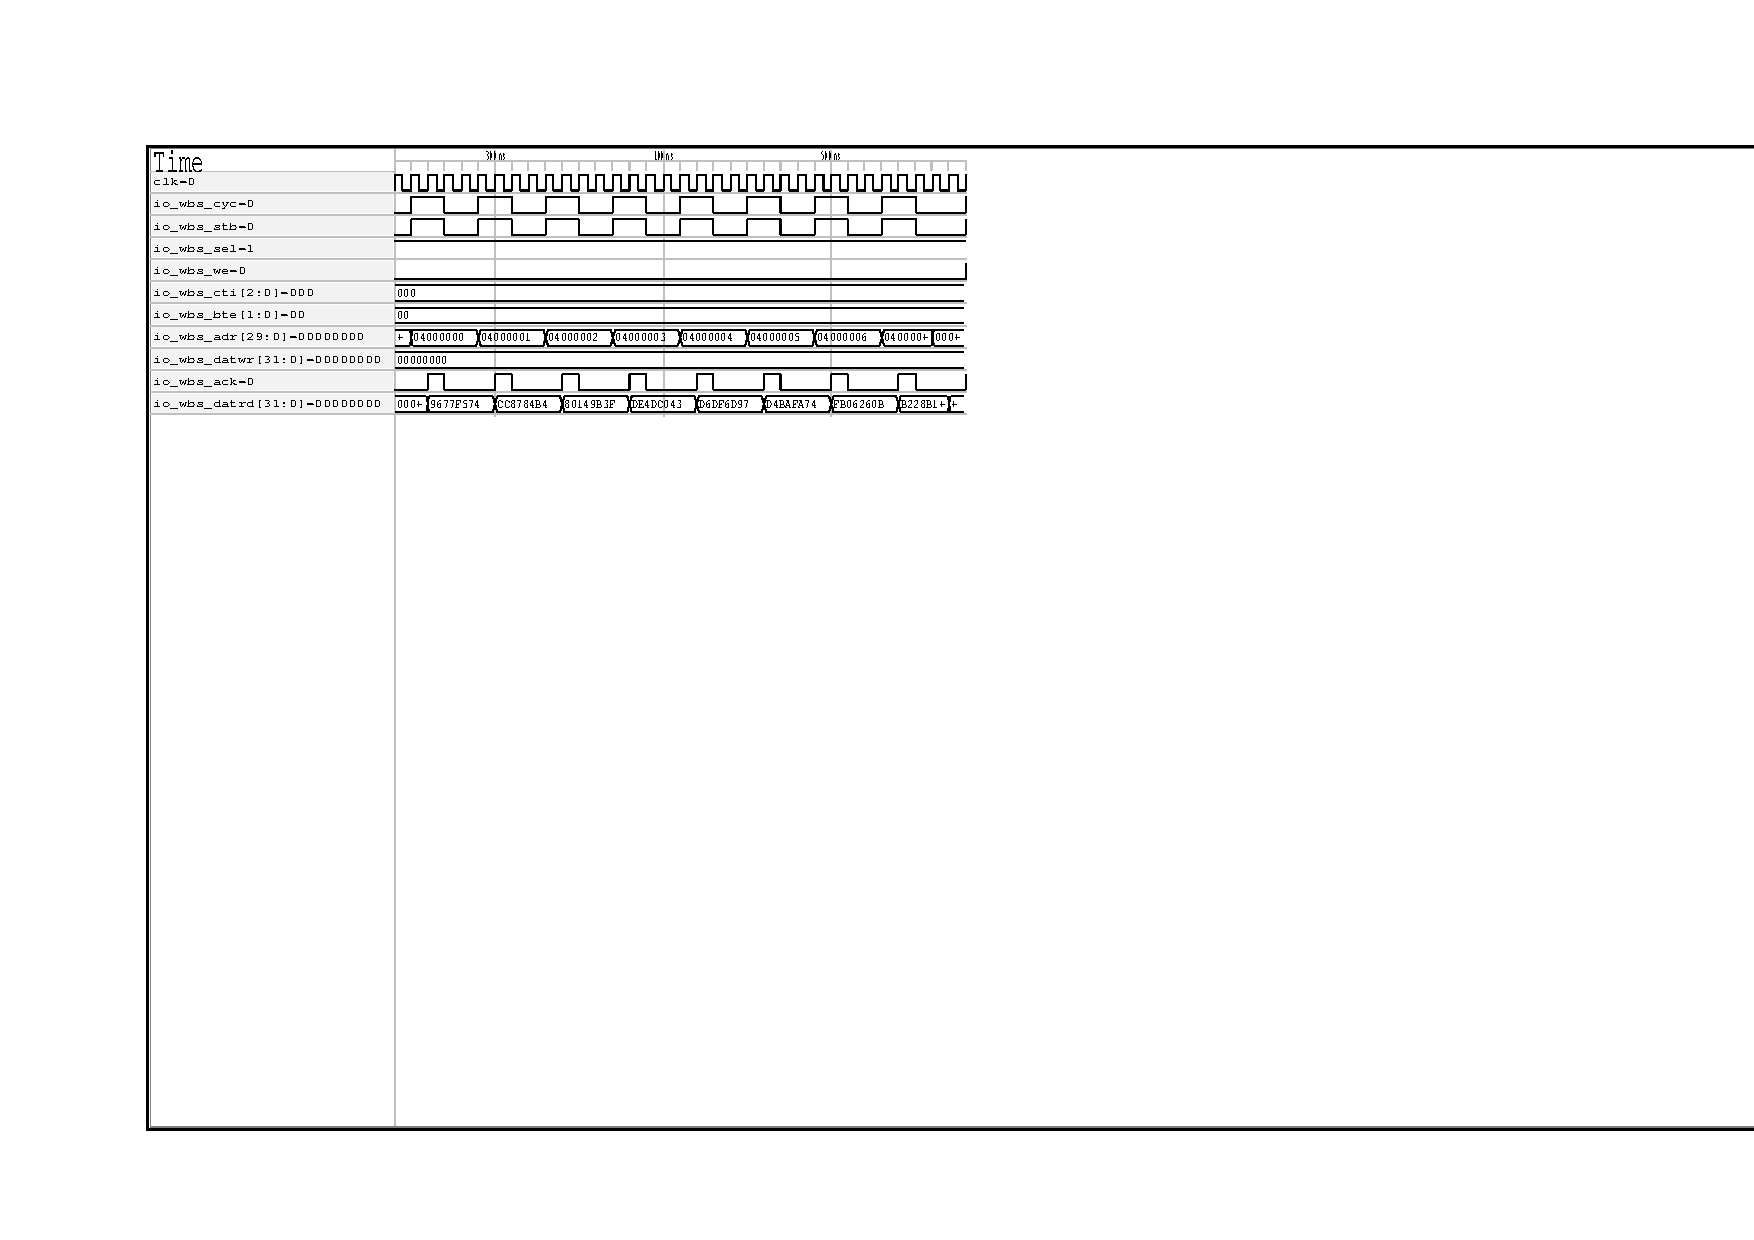
\includegraphics[scale=1,trim={2.54cm 14cm 13.4cm 2.9cm},clip]{testing/test-sram-classic-8.pdf}
	\caption{Przebieg odczytu danych z pamięci SRAM w klasycznym cyklu magistrali Wishbone}
	\label{fig:test-sram-classic-8}
\end{figure}

\begin{figure}[H]
	\centering
	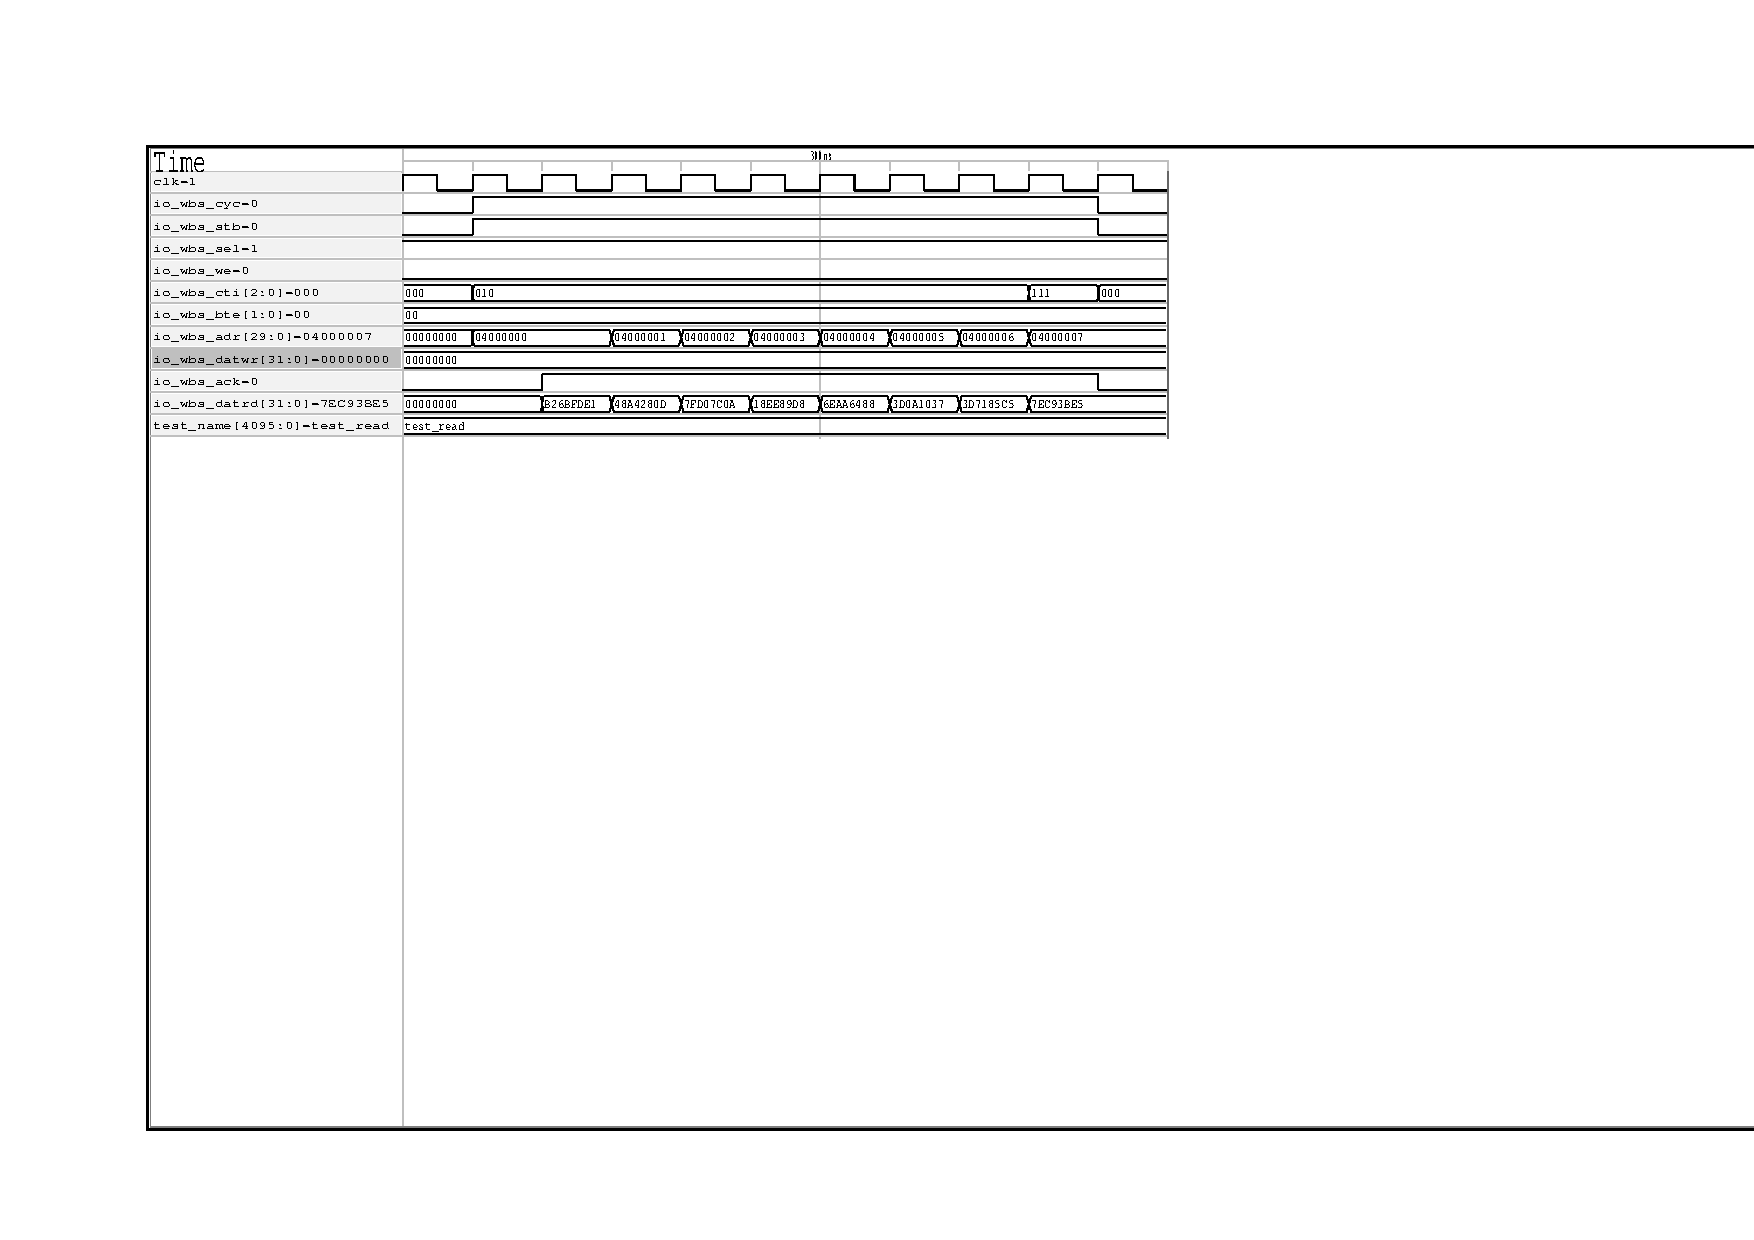
\includegraphics[scale=1,trim={2.54cm 14cm 11.2cm 2.9cm},clip]{testing/test-sram-increment-8.pdf}
	\caption{Przebieg odczytu danych z pamięci SRAM w cyklu potokowym z inkrementacją adresu magistrali Wishbone}
	\label{fig:test-sram-increment-8}
\end{figure}

Poprawność zapisanych danych została sprawdzona poprzez porównanie danych odczytanych poprzez magistralę ze zbiorem danych, które poprzednio zostały załadowane do pamięci z wykorzystaniem zewnętrznego portu. W przypadku cykli z inkrementacją adresu należy również sprawdzić, czy dane słowo zostało zachowane i odczytane w tym samym miejscu w pamięci, ze względu na inne zachowanie licznika adresu w interfejsie modułu SRAM przy inkrementacji adresu z użytym zawijaniem jego najmniej znaczących bitów. Z tego powodu testy wykorzystują dodatkowy parametr, który określa wartość dodaną do początkowego adresu, od którego zaczną się operacje na magistrali.

\begin{figure}[H]
	\centering
	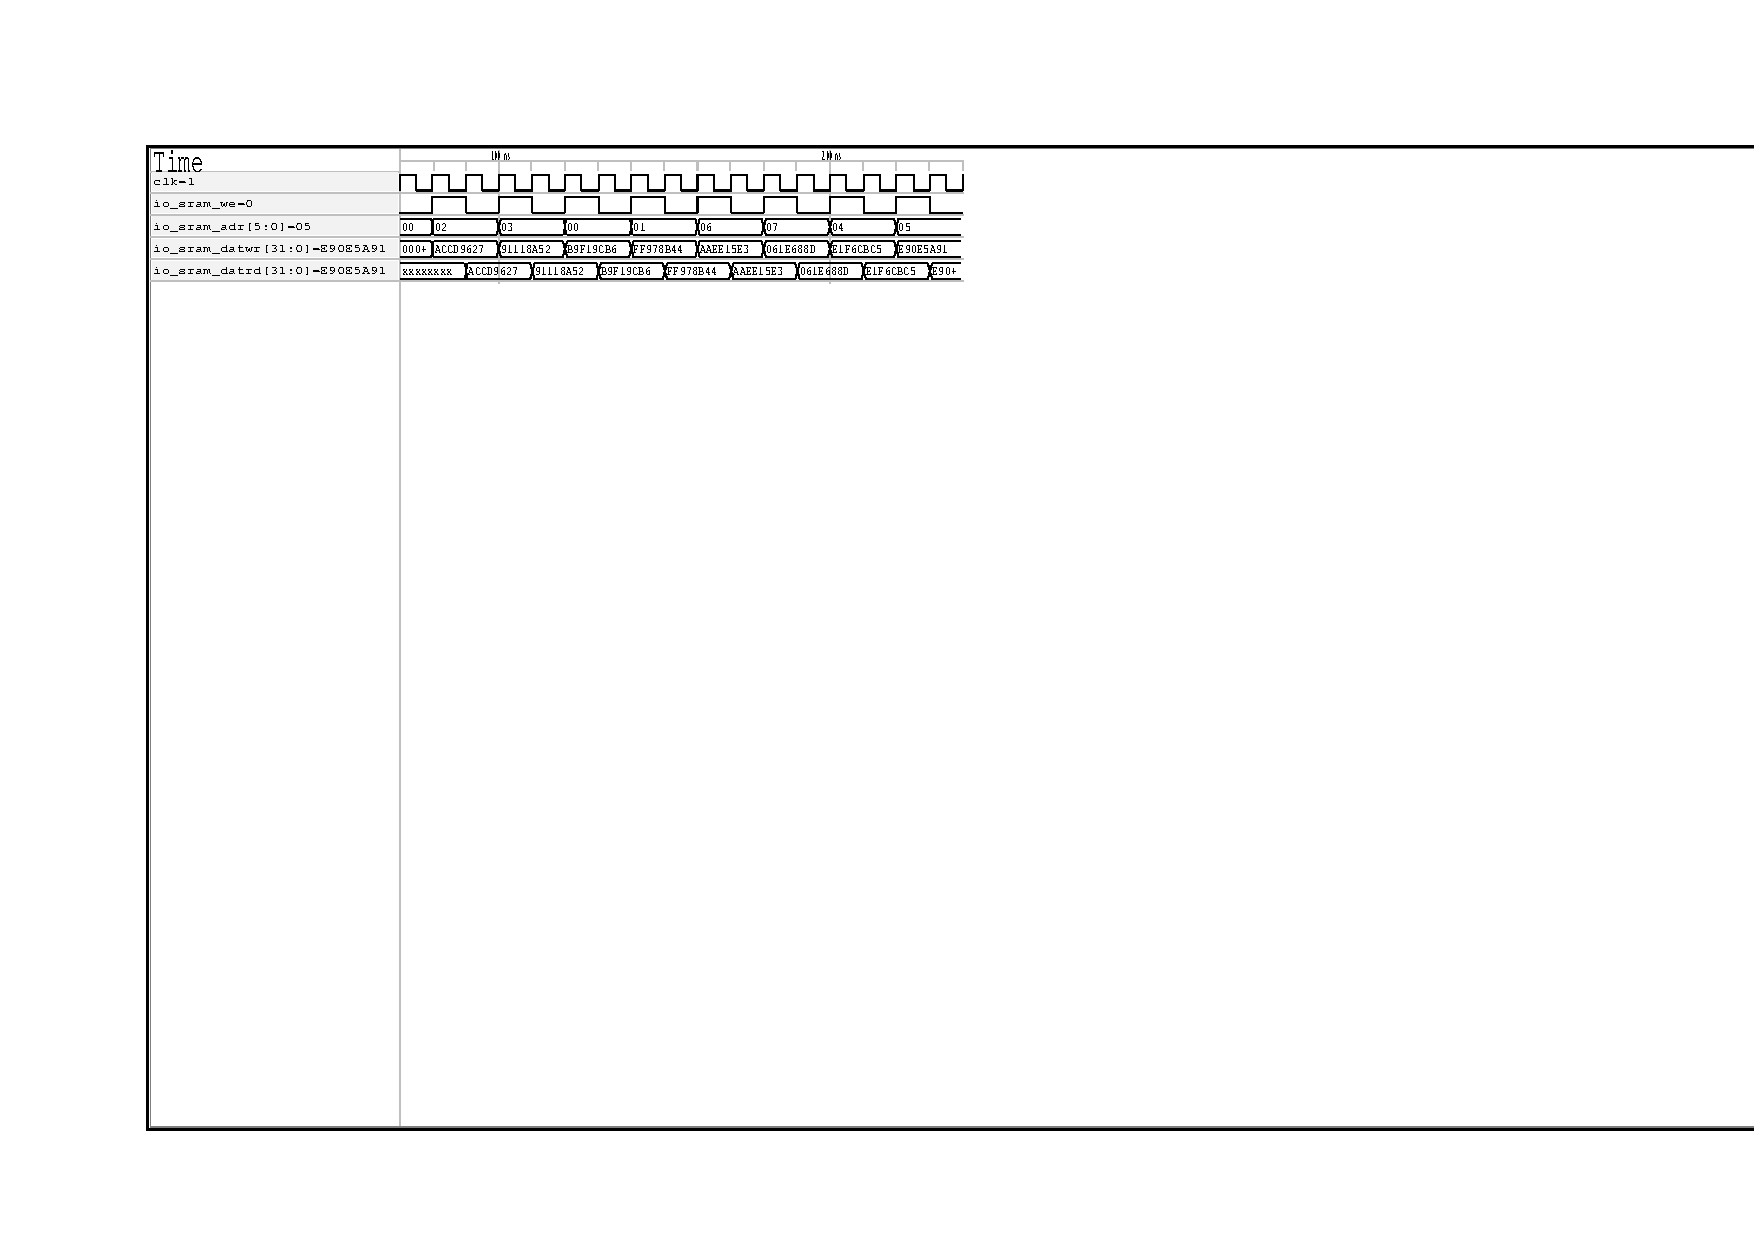
\includegraphics[scale=1,trim={2.54cm 16.2cm 12.3cm 2.9cm},clip]{testing/test-sram-valid-8-2.pdf}
	\caption{Przebieg zapisu testowych danych do pamięci SRAM z wykorzystaniem drugiego portu}
	\label{fig:test-sram-valid-8}
\end{figure}

\begin{figure}[H]
	\centering
	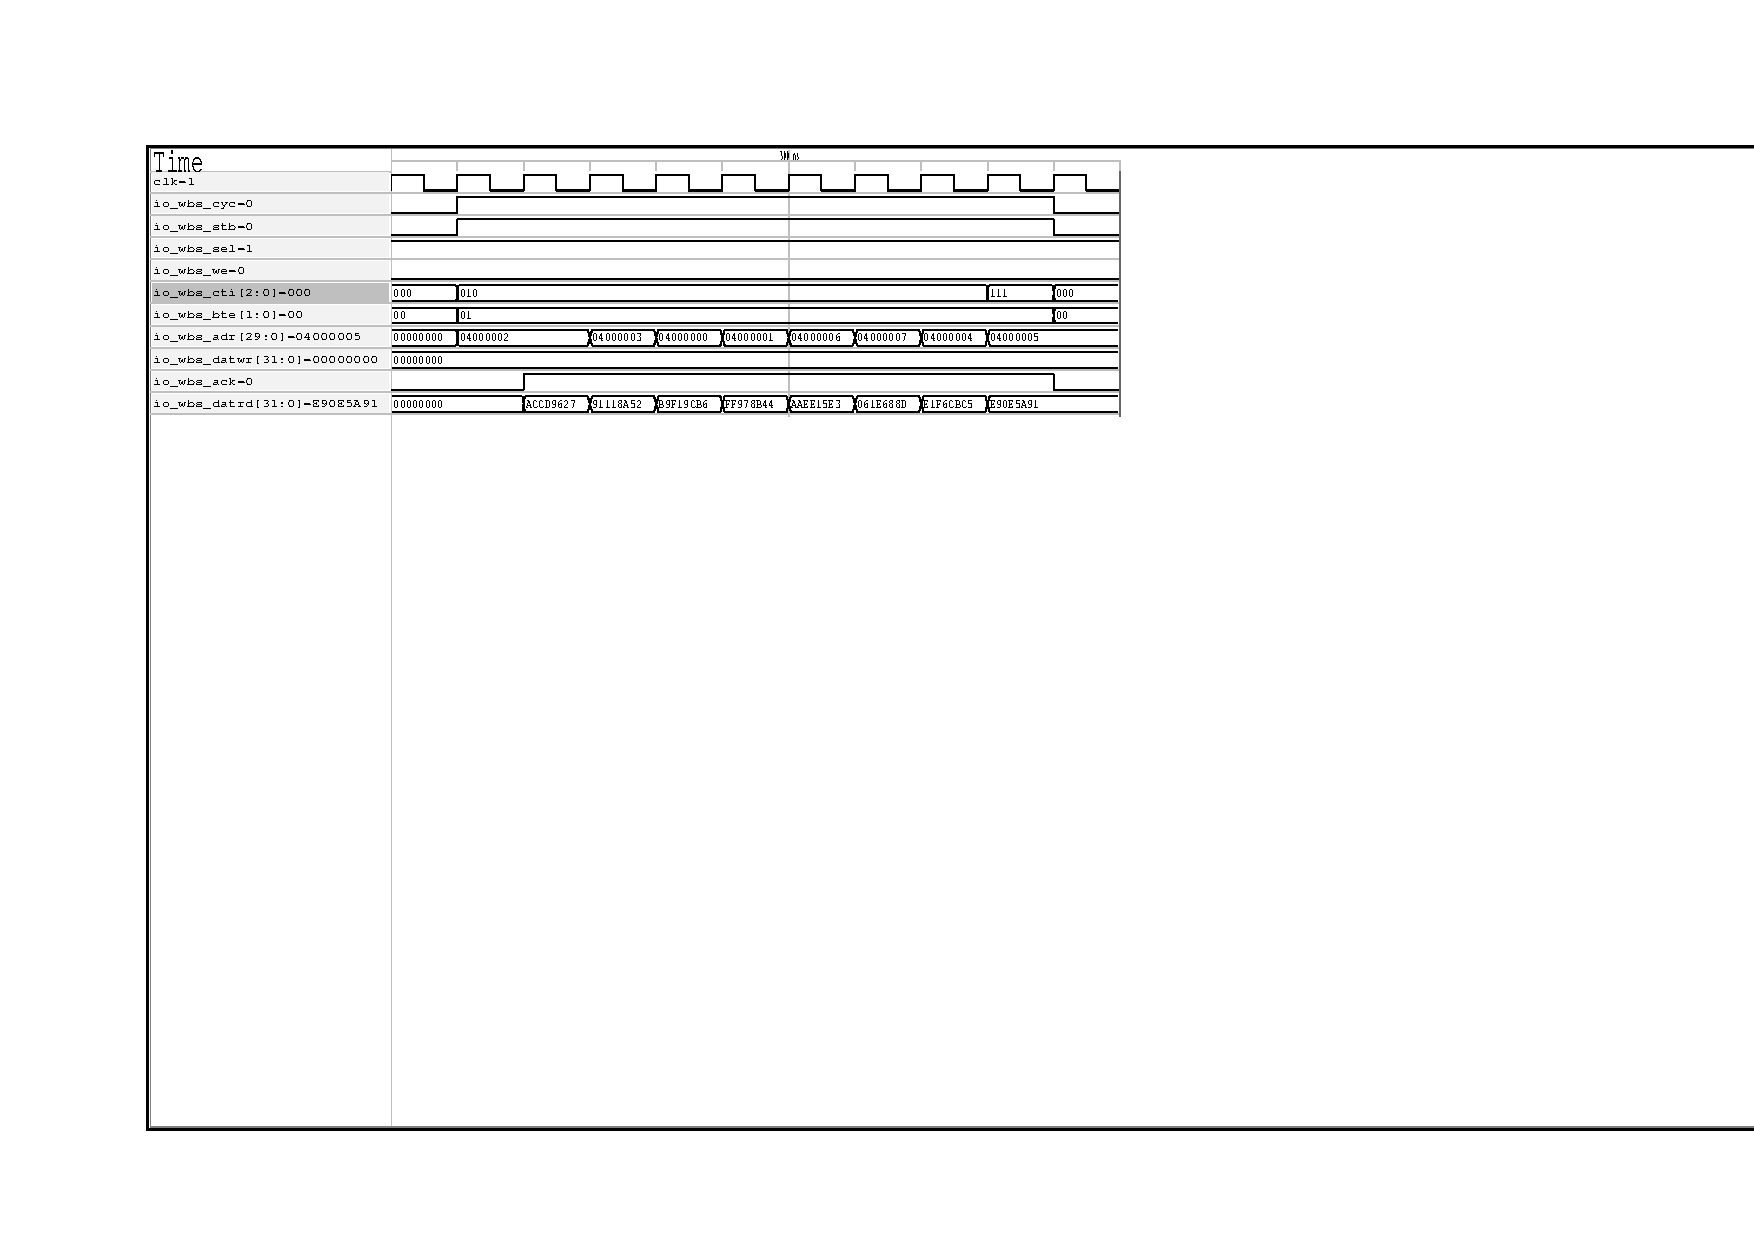
\includegraphics[scale=1,trim={2.54cm 14cm 11.3cm 2.9cm},clip]{testing/test-sram-wrapped-8-2.pdf}
	\caption{Przebieg odczytu danych z pamięci SRAM w cyklu potokowym z zawijaną inkrementacją adresu}
	\label{fig:test-sram-wrapped-8}
\end{figure}

Na przebiegu z rysunku \ref{fig:test-sram-wrapped-8} przedstawiony został odczyt ośmiu słów z parametrem \texttt{BTE} równym \texttt{0b01}. Wartość ta oznacza, że zawinięcie adresu obejmuje granicę czterech sąsiadujących ze sobą adresów. Odczyt danych poprzez magistralę rozpoczął się od adresu \texttt{0x002}. Po odczytaniu słowa z adresu \texttt{0x003} kolejne operacje następują na adresach \texttt{0x000}, \texttt{0x001} oraz \texttt{0x006}. Można zauważyć, że dwa najmniej znaczące bity adresów \texttt{0x002} i \texttt{0x006} są identyczne, co pokrywa się z założeniami mechanizmu zawiniętej inkrementacji adresu.
Po posortowaniu zapisanych i odebranych danych po ich adresach widoczne jest to, że są one identyczne. Oznacza to, iż dane zostały odczytane z tych samych adresów w pamięci SRAM, pod którymi zostały uprzednio zapisane w innej kolejności (zademonstrowane na przebiegu z rysunku \ref{fig:test-sram-valid-8}).

\subsection{Testy wydajnościowe systemu jednoukładowego na symulatorze oraz na układzie FPGA}

Po zweryfikowaniu poprawności działania peryferiów kolejnym etapem jest przeprowadzenie testów wydajnościowych. Polegać one będą na wykonaniu testowego układu SoC, który zawierać będzie peryferium w wariancie zarówno zmodyfikowanym, jak i oryginalnym. Na tym układzie uruchamiany będzie program, który będzie mierzyć prędkość operacji odczytu i zapisu zbioru danych w kolejności sekwencyjnej i losowej. Pozwoli to na zbadanie wpływu obsługi transferów potokowych na szybkość wykonywania operacji.

\subsubsection{Wykorzystane urządzenia}

Testy wydajnościowe były wykonywane w dwóch środowiskach: na przedstawionym na zdjęciu \ref{fig:arty-a7-photo} zestawie deweloperskim Digilent Arty A7-35\cite{digilent-arty-a7}, zawierającym układ programowalnych bramek logicznych Artix-7 firmy Xilinx, oraz na symulatorze uruchomionym na średniej klasy komputerze klasy PC będącym pod kontrolą systemu operacyjnego Debian GNU/Linux\cite{debian11}. Symulator został automatycznie zbudowany poprzez system LiteX z użyciem programu Verilator, natomiast plik konfigurujący zachowanie układu FPGA (zwany bitstreamem) zbudowany został z wykorzystaniem zbioru narzędzi do syntezy Vivado\cite{vivado2019.1} firmy Xilinx oraz, na potrzeby testowania kompatybilności, zestawu narzędzi F4PGA\cite{f4pga}.

\begin{figure}[H]
	\centering
	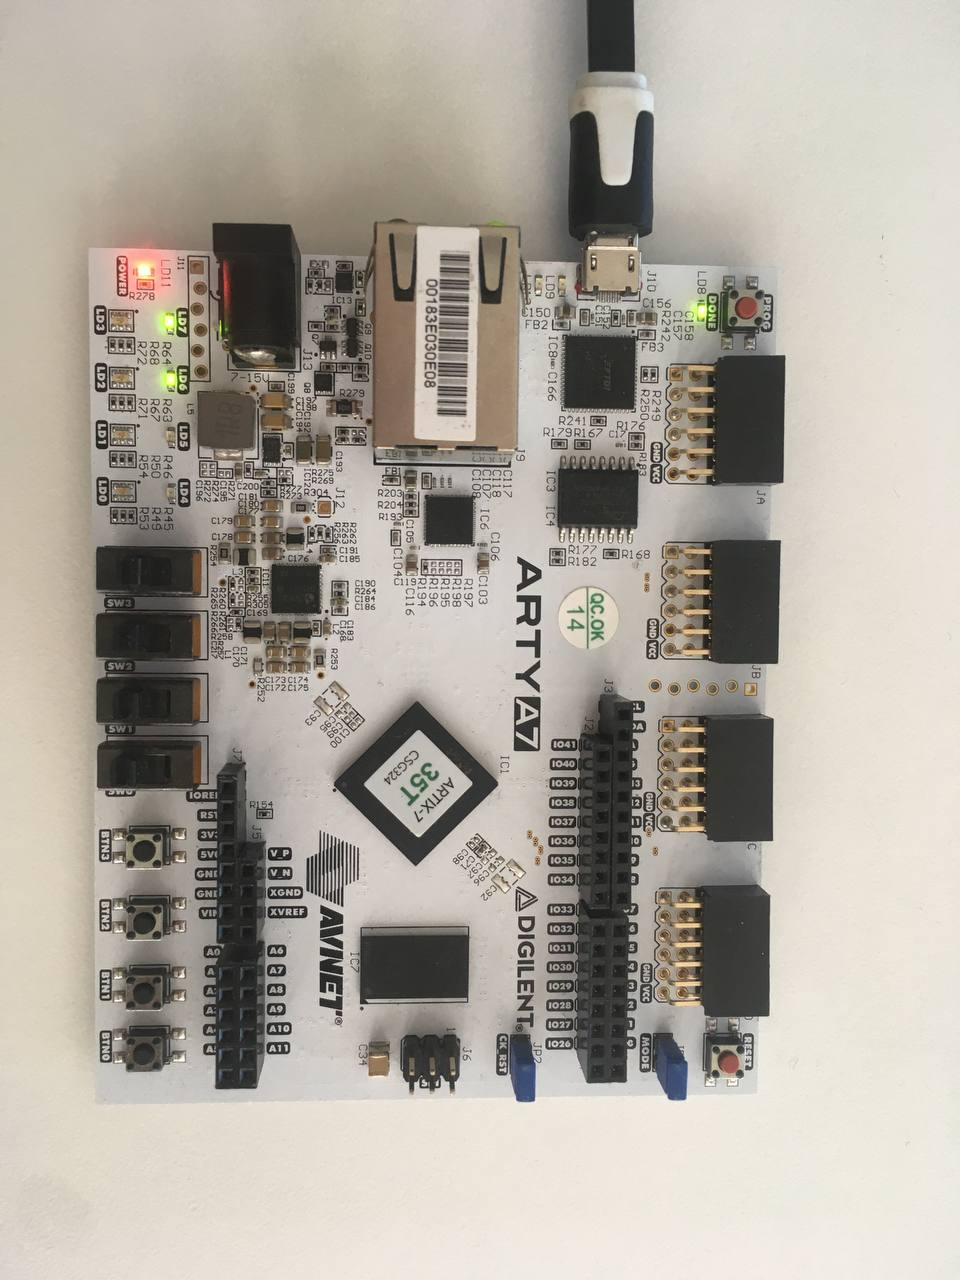
\includegraphics[angle=90,scale=0.3,trim={3cm 0 6cm 0},clip]{testing/photo_2022-09-16_13-47-42.jpg}
	\caption{Płytka deweloperska Digilent Arty-A7 z układem FPGA Xilinx Artix-7}
	\label{fig:arty-a7-photo}
\end{figure}

\subsubsection{Testowy układ SoC i jego architektura}

Testowy system mikroprocesorowy składa się z procesora VexRiscv, czterech bloków pamięci SRAM, interfejsu UART do komunikacji między programem testowym a użytkownikiem oraz niewykorzystanych bloków interfejsu Ethernet i analizatora stanów logicznych.
Procesor VexRiscv został skonfigurowany z pamięcią podręczną danych wielkości 4 kibibajtów oraz z obsługą architektury RV32I - obecność pamięci podręcznej jest szczególnie ważna, gdyż to właśnie na jej potrzeby procesor zawiera wsparcie dla transferów potokowych na magistrali Wishbone.
Z czterech pamięci SRAM dwa są w trybie tylko do odczytu --- zawierać będą program rozruchowy oraz program testowy, które załadowane będą jako część bitstreamu dla układu FPGA.

\begin{figure}[H]
	\centering
	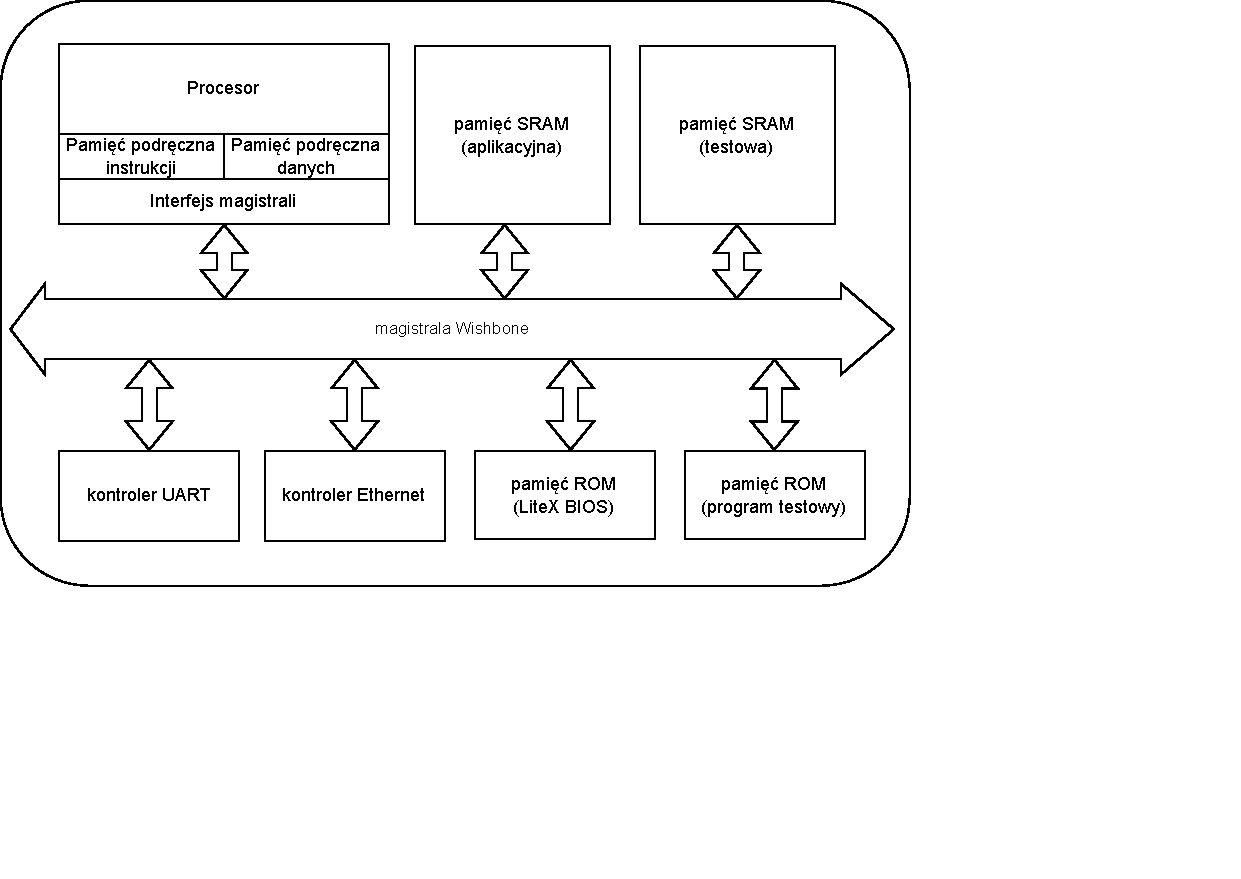
\includegraphics[scale=1,trim={0 4.9cm 5.6cm 0},clip]{testing/benchmark-soc-diag.pdf}
	\caption{Schemat blokowy układu SoC użytego do przeprowadzenia testów wydajnościowych}
	\label{fig:benchmark-soc-diag}
\end{figure}

\subsubsection{Program dla jednostki centralnej RISC-V badający szybkość operacji na pamięci}

Program testowy, zaimplementowany w języku C, testuje wybrany obszar pamięci poprzez zapisanie oraz odczytanie całego obszaru. Test ten jest wykonywany na dwa sposoby: dokonując operacji na kolejnych oraz losowych adresach.

\begin{listing}[H]
\begin{minted}{c}
int main(void)
{
#ifdef CONFIG_CPU_HAS_INTERRUPT
    irq_setmask(0);
    irq_setie(1);
#endif
    uart_init();

    printf("%s\n\n", MEM_REGIONS);
    printf(":%x@%p\n", TEST_SIZE, (void *)TEST_ADDR);

    puts(":A");
    memtest((unsigned int *)TEST_ADDR, TEST_SIZE);
    puts(":B");
    memspeed((unsigned int *)TEST_ADDR, TEST_SIZE, 0, 0);
    puts(":C");
    memspeed((unsigned int *)TEST_ADDR, TEST_SIZE, 0, 1);
    puts(":D");

    /* Finish simulation */
#ifdef CSR_SIM_FINISH_BASE
    sim_finish_finish_write(1);
#endif

    return 0;
}
\end{minted}
\caption{\label{lst:benchmark-main.c}Główna funkcja programu testowego służącego do pomiaru prędkości transferu danych}
\end{listing}

Funkcje odpowiadające za przeprowadzenie testu są dostępne w ramach biblioteki libbase, będącej częścią systemu LiteX --- o ile funkcje można wywołać z poziomu konsoli programu rozruchowego, to program na etapie budowania zapisuje adres startowy oraz pojemność testowanej pamięci przekazany przez skrypt budujący układ platformy testowej, pozwalając na automatyczne wykonanie testu w momencie załadowania bitstreamu na układ FPGA lub uruchomienia symulatora.
Dodatkową funkcjonalnością, dostępną w przypadku uruchomienia testu w symulacji, jest śledzenie wykonywania poprzez możliwość zapisywania flagi pod określonym wcześniej adresem --- zawartość tego adresu jest potem zapisywana w pliku z przebiegami sygnałów emulowanego systemu, dzięki czemu można zbadać, jakie operacje na magistrali są wykonywane w danym fragmencie testu.

\begin{figure}[H]
	\centering
	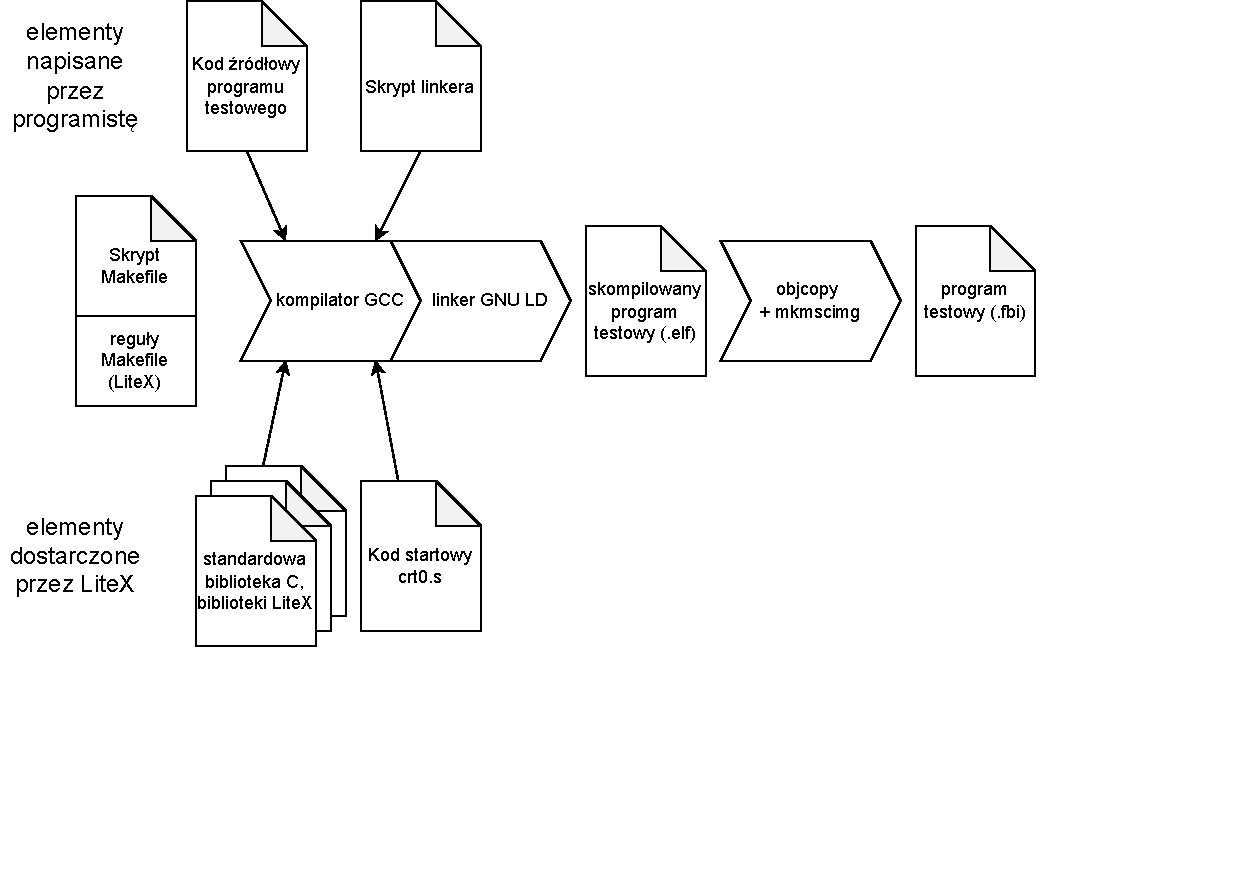
\includegraphics[scale=0.8,trim={0 3.9cm 3.5cm 0},clip]{testing/benchmark-program-pipeline.pdf}
	\caption{Proces budowania programu testowego}
	\label{fig:benchmark-program-pipeline}
\end{figure}

W celu skompilowania programu testowego użyty został kompilator GCC, skonfigurowany do emitowania kodu na platformę \texttt{riscv32-unknown-elf} - czyli 32-bitowego procesora RISC-V bez określonego systemu operacyjnego. Proces kompilacji, przedstawiony na rysunku \ref{fig:benchmark-program-pipeline}, jest opisany w pliku \texttt{Makefile}, który jest wywoływany przez skrypt budujący układ testowy. W czasie uruchamiania programu Make ustawiane są zmienne środowiskowe, które przechowują ścieżki do plików nagłówkowych definiujących adresy rejestrów w wygenerowanym układzie czy plik \texttt{crt0.s} dedykowany wybranemu głównemu procesorowi. Plik \texttt{crt0.s} przechowuje kod, którego zadaniem jest inicjalizacja pamięci programu przed przeskoczeniem do jego głównej procedury. Razem z kodem startowym i kodem programu testowego łączone są również biblioteki dostarczone przez system LiteX, wliczając w to standardową bibliotekę języka C.

Skompilowany program zostaje zapisany w pliku ELF, który oprócz samego kodu przechowuje informacje o wymaganych obszarach pamięci czy platformie, dla której przeznaczony jest ten program. Informacje te nie są wykorzystywane przez dołączony do systemu LiteX program rozruchowy o nazwie BIOS, który został skompilowany w czasie budowania układu testowego --- w tym celu z pliku ELF zostanie wyciągnięty fragment, który zawiera właściwy kod wykonywalny. Można tego dokonać z użyciem programu \texttt{objcopy}, który jest wywoływany automatycznie w skrypcie Makefile. Żeby BIOS jednak mógł załadować program testowy do głównej pamięci SRAM, na początku pliku musi być również informacja o rozmiarze kodu. Informacja zostaje dodana z użyciem skryptu \texttt{mkmscimg}, będącym jednym z narzędzi dostarczonym z systemem LiteX. Wynikowy plik z rozszerzeniem \texttt{.fbi} zostaje na koniec dodany jako zawartość aplikacyjnej pamięci ROM wygenerowanego układu.

\subsubsection{Wyniki testów wydajnościowych}

Testy zostały wykonane kilkukrotnie, ich wyniki zaś uśrednione w celu otrzymania lepszej powtarzalności wyników w konkretnym środowisku.

Dla programu testowego uruchomionego w symulatorze Verilator na średniej klasy komputerze osobistym z symulowaną prędkością 1 MHz wyniki prezentują się następująco:

\begin{center}

\begin{table}[H]
\begin{tabular}{ r|l|l|l| }
  & prędkość bazowa & prędkość po zmianach & różnica względem prędkości bazowej\\
 \hline
 zapis & 1.6 MiB/s & 1.6 MiB/s & 100.0\%\\
 odczyt & 918.3 KiB/s & 1.1 MiB/s & 123.6\%\\
 \hline
\end{tabular}
\caption{\label{tab:benchmark-seq-sim}Wyniki pomiaru prędkości operacji sekwencyjnych na symulowanej platformie testowej}
\end{table}

\begin{table}[H]
\begin{tabular}{ r|l|l|l| }
  & prędkość bazowa & prędkość po zmianach & różnica względem prędkości bazowej\\
 \hline
 zapis & 1.6 MiB/s & 1.6 MiB/s & 100.0\%\\
 odczyt & 122.7 KiB/s & 154.8 KiB/s & 126.2\%\\
 \hline
\end{tabular}
\caption{\label{tab:benchmark-rnd-sim}Wyniki pomiaru prędkości operacji losowych na symulowanej platformie testowej}
\end{table}

\end{center}

Ten sam program uruchomiony na platformie zrealizowanej z wykorzystaniem układu FPGA taktowanego zegarem 100 MHz natomiast pokazuje następujące rezultaty:

\begin{table}[H]
\begin{center}
\begin{tabular}{ r|l|l|l| }
  & prędkość bazowa & prędkość po zmianach & różnica względem prędkości bazowej\\
 \hline
 zapis & 166.6 MiB/s & 1.6 MiB/s & 100.0\%\\
 odczyt & 87.2 MiB/s & 110.4 MiB/s & 126.6\%\\
 \hline
\end{tabular}
\end{center}
\caption{\label{tab:benchmark-seq-arty}Wyniki pomiaru prędkości operacji sekwencyjnych na układzie FPGA}
\end{table}

\begin{table}[H]
\begin{center}
\begin{tabular}{ r|l|l|l| }
  & prędkość bazowa & prędkość po zmianach & różnica względem prędkości bazowej\\
 \hline
 zapis & 166.6 MiB/s & 166.7 MiB/s & 100.0\%\\
 odczyt & 11.6 MiB/s & 14.7 MiB/s & 126.6\%\\
 \hline
\end{tabular}
\end{center}
\caption{\label{tab:benchmark-rnd-arty}Wyniki pomiaru prędkości operacji losowych na układzie FPGA}
\end{table}

Na podstawie wyników można zauważyć, iż prędkość odczytu z pamięci wzrosła o 23 do 26 punktów procentowych względem prędkości platformy bez obsługi transferów potokowych. Oznacza to, iż wdrożone modyfikacje przyspieszyły odczyt danych w znaczącym stopniu bez konieczności przyspieszenia taktowania całego układu.

Brak zmian w prędkości zapisu można wytłumaczyć tym, iż procesor wykonywuje kilka operacji, zanim pojedyncze słowo będzie gotowe do zapisania w pamięci --- tym samym transfery potokowe nie zachodzą, gdyż nie jest możliwym przygotowanie nowych słów w każdym kolejnym takcie zegara.
Podobnie można wytłumaczyć również zmianę w prędkości odczytu --- procesor w jednym cyklu potokowym odczytuje tyle słów, ile można zmieścić w pojedynczej linii pamięci podręcznej. Dzięki temu procesor szybciej może pobrać dane z kilku sąsiadujących adresów. Przy bardziej odległych od siebie adresach procesor musi jednak ponownie pobrać dane bezpośrednio z pamięci RAM, gdyż nie zostały one załadowane do pamięci podręcznej przy poprzedniej operacji odczytu potokowego.

\subsection{Wnioski po realizacji testów}

Testy napisane na potrzeby tego projektu pozwoliły na pokrycie każdego rodzaju cyklu transferu danych na magistrali, co pozwoliło na zweryfikowane poprawności implementacji transferów potokowych. Parametryzacja testów pozwoliła zaś na weryfikację, czy dla różnych kombinacji warunków początkowych cyklu mechanizm działał poprawnie, ułatwiając wyszukiwanie błędów ujawniających się tylko przy określonych kombinacjach parametrów. Ułatwiło to zwłaszcza testowanie cyklów potokowych z zawijającą inkrementacją adresów, gdzie zachowanie licznika różniło się w zależności od wybranego rozmiaru zawinięcia oraz najmniej znaczących bitów adresu, od którego rozpoczął się cykl transferu.

Wyniki osiągnięte programem mierzącym prędkość transferu danych uruchomionym na testowym systemie jednoukładowym zademonstrowały średni wzrost wydajności o co najmniej 23 procent. Jest to zadowalający wynik względem wysiłku włożonego w zaimplementowanie wsparcia transferów potokowowych w module pamięci SRAM bez wprowadzania optymalizacji w innych fragmentach systemu czy oprogramowania testowego.
